\begin{mydef}
	La mesure (distance entre ses deux extrémités) d'un segment est sa \kw{longueur}.
\end{mydef}

\begin{myprop}
	La longueur d'un segment $[AB]$, se note $AB$ ou $BA$. 
\end{myprop}

\begin{myex}
	\vspace*{-0.5cm}
	\begin{center}
		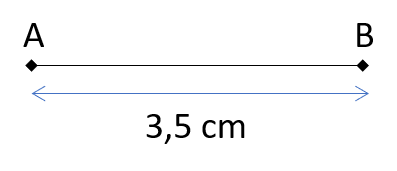
\includegraphics[scale=0.8]{img/lgr}
	\end{center}
	\vspace*{-0.5cm}
	La longueur du segment $[AB]$ est de \num{3.5} cm, on note
\end{myex}

\begin{mydef}
	Le \kw{milieu} d'un segment est le point qui appartient au segment \kw{et} qui est à égale distance de ses extrémités.
\end{mydef}

\begin{myrem}
	Des segments de même longueur sont codés de façon identique.
\end{myrem}

\begin{myex}
	\begin{center}
		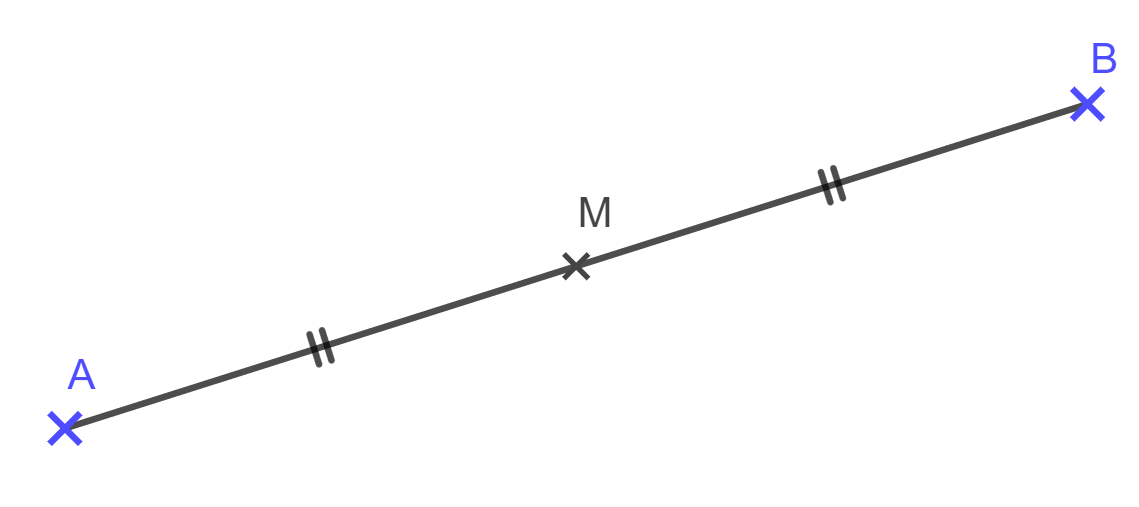
\includegraphics[scale=0.25]{img/milieu}
	\end{center}

	On a : $M \in [AB]$ et $AM = MB$, donc le point $M$ est le milieu du segment $[AB]$. On a ainsi $AM = AB \div 2$. 
\end{myex}